\section{Cours 1}\label{cours-1}

\subsection{Fondamentaux}\label{fondamentaux}

On a des composants:

\begin{itemize}
\tightlist
\item
  RAM, CPU, IO devices, \ldots{}
\end{itemize}

Le processeur exécute des \emph{instructions}.

\begin{itemize}
\tightlist
\item
  Lire / écrire en mémoire vers / depuis des registres
\item
  Opérations sur ces registres
\end{itemize}

Il y a 2 grandes familles \emph{X86\_64} et \emph{ARM A64} avec des jeux
d'instructions différents.

\subsubsection{Architecture de von
Neumann}\label{architecture-de-von-neumann}

\begin{figure}
\centering
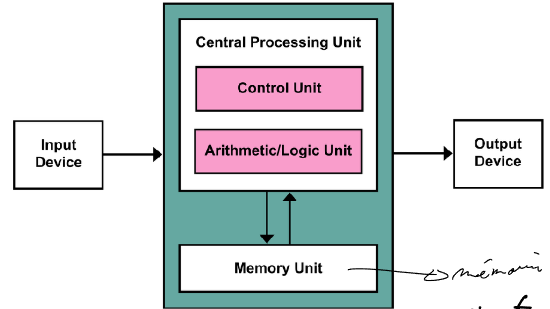
\includegraphics{image-5.png}
\caption{alt}
\end{figure}

\subsection{Représentation des
données}\label{repruxe9sentation-des-donnuxe9es}

On a typiquement:

\begin{longtable}[]{@{}cc@{}}
\toprule\noalign{}
taille & nom \\
\midrule\noalign{}
\endhead
\bottomrule\noalign{}
\endlastfoot
4 bits & nibble \\
8 bits & octet \\
32 bits & mot \\
64 bits & long mot \\
\end{longtable}

\subsection{Fonctionnement d'un système
informatique}\label{fonctionnement-dun-systuxe8me-informatique}

Les opérations d'entrée/sortie se déroulent de manière
\emph{concurrente}. Chacun a un contrôleur qui a une mémoire spécifique.
Le processeur doit transporter les infos de la mémoire classique à la
zone des contrôleurs.

Un processeur n'est pas de base parallélisé. À chaque frappe du clavier,
une \textbf{interruption} est lancée pour intercepter ce stimulis.

\subsubsection{Interruption}\label{interruption}

Le processeur va s'arrêter dans son exécution et va \emph{transférer} le
contrôle du processeur à une routine de traitement.

La routine de traitement va déterminer la source de l'interruption

Il va positionner le compteur de programme à la \emph{première}
exécution du segment de code associé à cette \emph{source}.

À la fin du traitement, on restaure l'état du processeur et on reprend
le processus interrompu en restaurant le compteur de programme

\subsection{Opérations
d'entrée/sorite}\label{opuxe9rations-dentruxe9esorite}

\begin{figure}
\centering
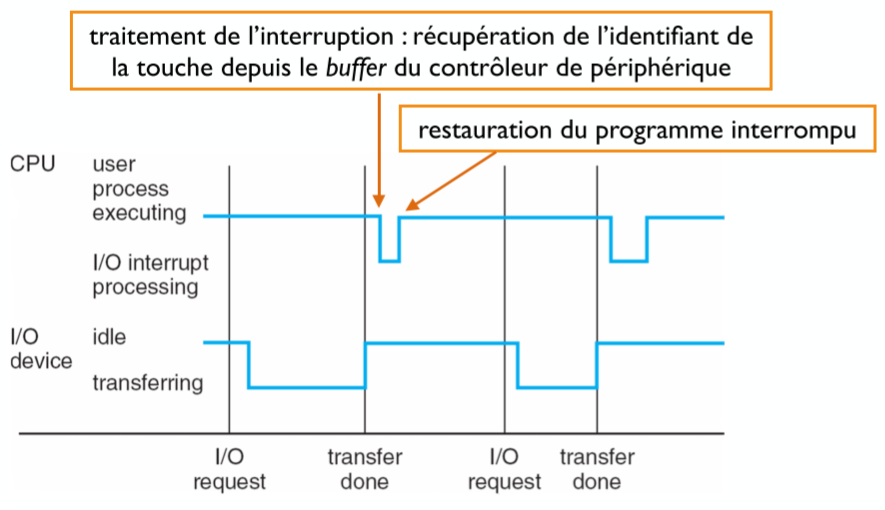
\includegraphics{image.png}
\caption{Alt text}
\end{figure}

\subsection{Accès direct à la
mémoire}\label{accuxe8s-direct-uxe0-la-muxe9moire}

Pour chaque touche de clavier, on doit interrompre pour que le
processeur utilise ces données.

Pour éviter les interruptions qui vont à l'infini, on utilise du
\textbf{DMA} qui est \emph{l'accès direct à la mémoire}. Cela permet un
transfert direct entre le contrôleur de périphérique et la mémoire
principale.

\begin{figure}
\centering
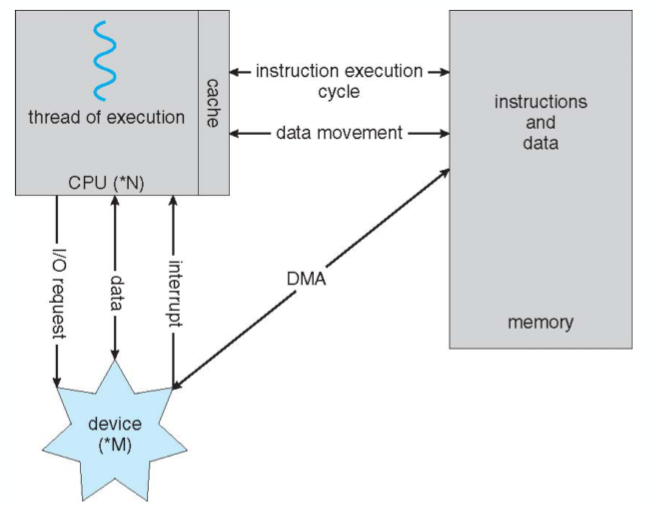
\includegraphics{image-1.png}
\caption{Alt text}
\end{figure}

\subsection{Le rôle du système
d'exploitation}\label{le-ruxf4le-du-systuxe8me-dexploitation}

Le système d'exploitation se met entre l'utilisateur et le matériel. Il
a 3 rôles:

\begin{enumerate}
\def\labelenumi{\arabic{enumi}.}
\tightlist
\item
  Rendre plus simple le développement de programmes
\item
  Utilisation plus efficaces des ressources
\item
  Assurer l'intégrité des données et des programmes entre eux.
\end{enumerate}

\subsection{Virtualisation}\label{virtualisation}

Le système d'exploitation assure cela en \textbf{virtualisant} les
ressources matérielles. On va donc utiliser des API,\ldots{}

\subsubsection{Exemple}\label{exemple}

\begin{itemize}
\tightlist
\item
  Processus
\item
  Le programmeur a l'impression d'avoir tout le processeur
\item
  Processus coexiste et s'entremêle
\item
  Partage du temps et des ressources
\item
  Virtualisation de la mémoire

  \begin{itemize}
  \tightlist
  \item
    Plusieurs processus en mémoire.
  \item
    On empêche que les autres processus lisent la mémoire des autres
  \item
    Le SE gère la correspondance entre les adresses de la mémoire
    \emph{virtuelle} et les addresses physiques
  \end{itemize}
\end{itemize}

\subsection{Compromis
abstraction/coût}\label{compromis-abstractioncouxfbt}

Cela facilite énormément la vie du programmeur.

\textbf{Mais} on doit à chaque fois recalculer et cela coûte cher en
calcul.

\textbf{Cependant} on a pu réduire ce coût de calcul via l'ajout de
fonctionnalités aux processeurs.

\subsection{Séparation entre mécanisme et
politique}\label{suxe9paration-entre-muxe9canisme-et-politique}

Via la virtualisation par exemple:

\begin{enumerate}
\def\labelenumi{\arabic{enumi}.}
\tightlist
\item
  Mécanisme de partage de temps:

  \begin{itemize}
  \tightlist
  \item
    Changement de contexte: sauvegarde l'état du processeur et restaure
  \end{itemize}
\item
  Politique arbitre entre les processeurs pouvant s'exécuter et les
  processeurs disponibles:

  \begin{itemize}
  \tightlist
  \item
    Politique d'ordonnancement (\emph{scheduling})
  \end{itemize}
\end{enumerate}

On peut donc changer les \emph{politiques d'ordonnancement} différentes
selon les besoins mais avec le même mécanisme.

\subsection{Modes d'exécution}\label{modes-dexuxe9cution}

\begin{itemize}
\tightlist
\item
  \textbf{Utilisateur}: programme utilisant les abstractions fournies
  par le SE.
\item
  \textbf{Protégé}: utilisé par le noyau du SE, toutes les instructions
  sont autorisées
\end{itemize}

L'utilisation de fonctionnalités du SE par un processus utilisateur
nécessite de passer d'un mode à l'autre. (\emph{appel système})

\subsection{Appel système ==
interruption}\label{appel-systuxe8me-interruption}

\begin{figure}
\centering
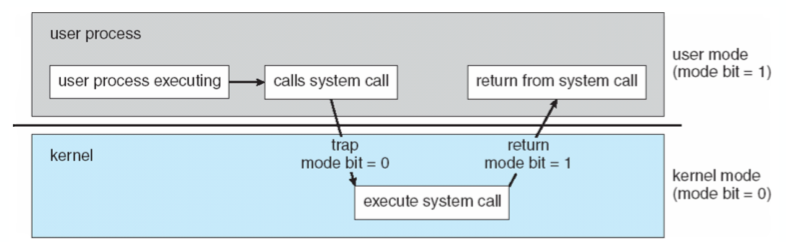
\includegraphics{image-2.png}
\caption{Alt text}
\end{figure}

\subsection{En Résume}\label{en-ruxe9sume}

Système d'exploitation \textasciitilde= traitement des interruptions

\begin{itemize}
\tightlist
\item
  Interruptions matérielles (IO)
\item
  Interruptions du processeur (instructions illégales user)
\item
  Interruptions logicielles (appels systèmes)
\end{itemize}

\subsection{UNIX}\label{unix}

Est une famille de système d'exploitation.

Ici, on verra surtout GNU/Linux. - Linux: kernel - GNU: collection
d'utilitaires et de librairies associés.

\begin{figure}
\centering
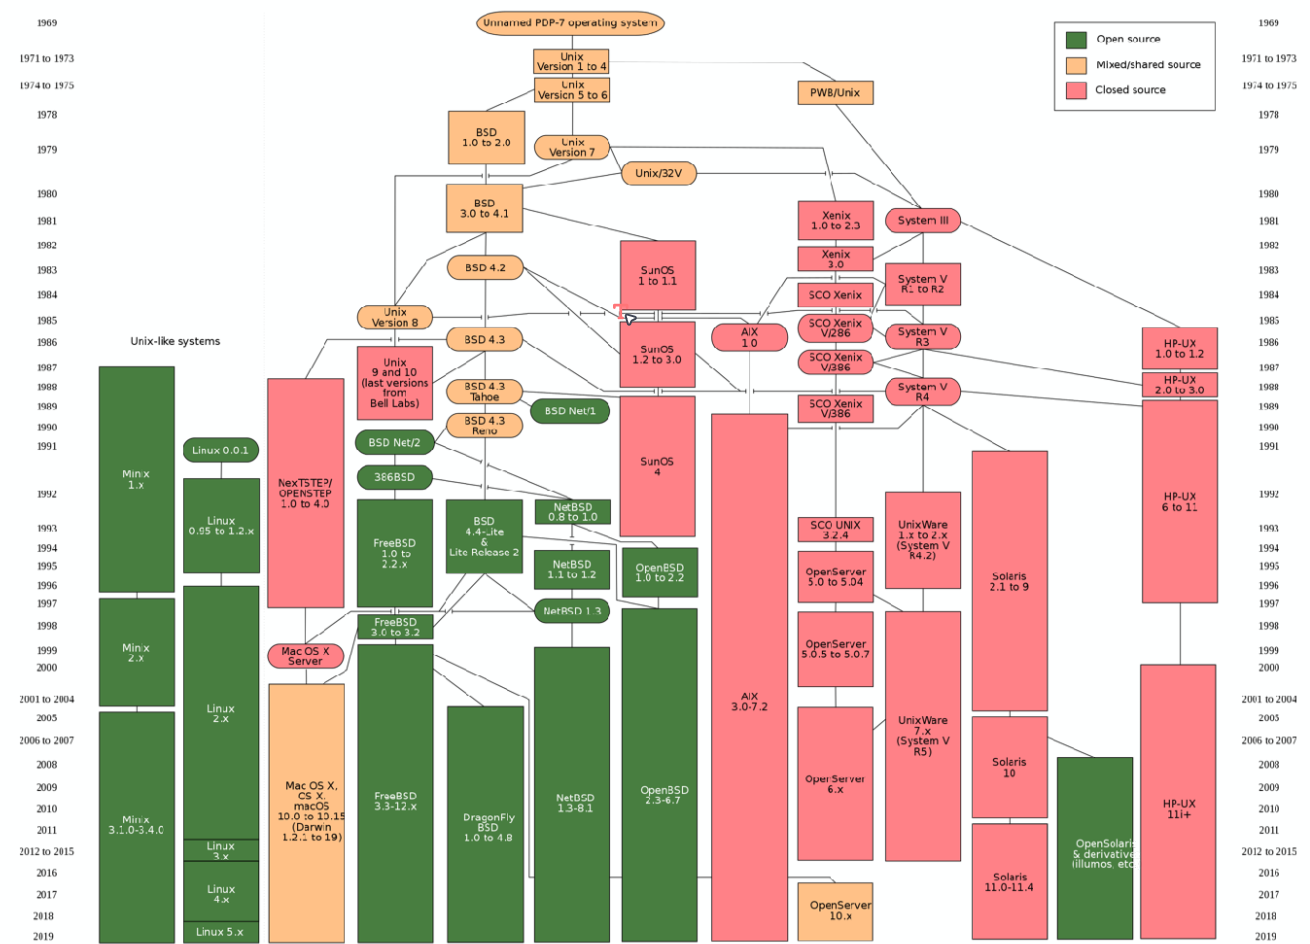
\includegraphics{image-3.png}
\caption{La grande famille UNIX}
\end{figure}

Il y a la philosophie \emph{KISS}:

\begin{itemize}
\tightlist
\item
  \emph{Keep It Simple, Stupid}
\item
  Programme simple, petit, parfaitement adapté à une tâche ou fonction
  unique
\item
  Facilité de composition de commandes
\end{itemize}

\begin{longtable}[]{@{}
  >{\centering\arraybackslash}p{(\columnwidth - 2\tabcolsep) * \real{0.1134}}
  >{\centering\arraybackslash}p{(\columnwidth - 2\tabcolsep) * \real{0.8866}}@{}}
\toprule\noalign{}
\begin{minipage}[b]{\linewidth}\centering
Utilitaire
\end{minipage} & \begin{minipage}[b]{\linewidth}\centering
Fonction
\end{minipage} \\
\midrule\noalign{}
\endhead
\bottomrule\noalign{}
\endlastfoot
cat & lire/afficher le contenu d'un fichier. ex :
\texttt{cat\ fichier.txt} \\
echo & afficher une chaîne de caractère \\
head / tail & affiche le début ou la fin d'un fichier \\
wc & compte le nombre de caractères \\
sort & trie un fichier. ex:\texttt{sort\ -n\ -r\ scores.txt} \\
uniq & extrait les lignes uniques ou dupliquées d'un fichier trié. ex:
\texttt{uniq\ -d\ students.dat} \\
\end{longtable}

\subsection{La documentation}\label{la-documentation}

Chaque utilitaire possède une manpage.

\texttt{man\ nom\_utilitaire}

On a des sections de manuelles qui différencient et trient les
utilitaires (librairie standard, appel système, \ldots)

\begin{enumerate}
\def\labelenumi{\arabic{enumi}.}
\tightlist
\item
  Utilitaires disponibles pour tous les utilisateurs
\item
  Appels systèmes en C
\item
  Fonctions de la librairie
\item
  Fichiers spéciaux
\item
  Formats de fichiers et conventions pour certains types de fichiers
\item
  Jeux
\item
  Utilitaires de manipulation de fichier textes
\item
  Commandes et procédure de gestion du système
\end{enumerate}

Donc parfois on doit préciser \texttt{man\ 1\ printf}.

\subsection{Flux standards}\label{flux-standards}

\begin{figure}
\centering
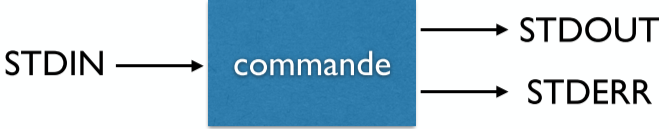
\includegraphics{image-4.png}
\caption{Flux}
\end{figure}

On a 1 entrées, 1 sorties par défaut dans le shell (STDOUT) et une
sortie d'erreur (STDERR)

\begin{longtable}[]{@{}
  >{\centering\arraybackslash}p{(\columnwidth - 2\tabcolsep) * \real{0.1139}}
  >{\centering\arraybackslash}p{(\columnwidth - 2\tabcolsep) * \real{0.8861}}@{}}
\toprule\noalign{}
\begin{minipage}[b]{\linewidth}\centering
commande
\end{minipage} & \begin{minipage}[b]{\linewidth}\centering
action
\end{minipage} \\
\midrule\noalign{}
\endhead
\bottomrule\noalign{}
\endlastfoot
\texttt{\textless{}\ file} & redirige le contenu de \texttt{file} vers
STDIN \\
\texttt{\textgreater{}\ file} & redirige STDOUT vers \texttt{file} \\
\texttt{\textgreater{}\textgreater{}\ file} & redirige STDOUT vers
\texttt{file} et l'ajoute au bout d'un fichier si existe \\
\texttt{2\textless{}\&1} & redirige STDERR vers STDOUT \\
\end{longtable}

On a aussi des Pipes qui redirige le résultat de commande de STDOUT vers
le STDIN d'une autre commande.

\begin{Shaded}
\begin{Highlighting}[]
\ExtensionTok{cmd1} \KeywordTok{|} \ExtensionTok{cmd2}
\end{Highlighting}
\end{Shaded}

\subsection{Script}\label{script}

En entête de script \emph{interprété} il faut ajouter l'interpréteur
(python, bash):

\begin{Shaded}
\begin{Highlighting}[]
\CommentTok{\#!/bin/bash}
\BuiltInTok{echo} \StringTok{"Hello, world"}
\end{Highlighting}
\end{Shaded}

\subsubsection{Arguments en ligne de
commande}\label{arguments-en-ligne-de-commande}

\begin{Shaded}
\begin{Highlighting}[]
\CommentTok{\#!/bin/bash }
\CommentTok{\# $\# nombre d\textquotesingle{}arguments }
\CommentTok{\# $1 $2 $3 ... arguments }
\BuiltInTok{echo} \StringTok{"Vous avez passé"} \VariableTok{$\#} \StringTok{"arguments"} 
\BuiltInTok{echo} \StringTok{"Le premier argument est :"} \VariableTok{$1}
\BuiltInTok{echo} \StringTok{"Liste des arguments :"} \VariableTok{$@}
\end{Highlighting}
\end{Shaded}

\subsubsection{Retour}\label{retour}

On peut retourner le résultat de la dernière commande via \texttt{\$?}.
Si 0 c'est bon.

On peut envoyer des données dans \texttt{/dev/null} et c'est un trou
noir.

On peut lire du contenu aléatoire dans \texttt{/dev/random}.

\subsubsection{\texorpdfstring{Boucles
\texttt{for}}{Boucles for}}\label{boucles-for}

\begin{Shaded}
\begin{Highlighting}[]
\CommentTok{\#!/bin/bash }
\CommentTok{\# exemple\_for.sh }
\VariableTok{students}\OperatorTok{=}\StringTok{"Julie Maxime Hakim"} 
\ControlFlowTok{for}\NormalTok{ s }\KeywordTok{in} \VariableTok{$students}\KeywordTok{;} \ControlFlowTok{do} 
  \VariableTok{l}\OperatorTok{=}\KeywordTok{\textasciigrave{}}\FunctionTok{wc} \AttributeTok{{-}l}\NormalTok{ TP1{-}}\VariableTok{$s}\NormalTok{.txt }\KeywordTok{|} \FunctionTok{cut} \AttributeTok{{-}d}\StringTok{\textquotesingle{} \textquotesingle{}} \AttributeTok{{-}f1}\KeywordTok{\textasciigrave{}} 
  \BuiltInTok{echo} \StringTok{"Bonjour }\VariableTok{$s}\StringTok{, ton compte rendu de TP comporte }\VariableTok{$l}\StringTok{ lignes."}
\ControlFlowTok{done}
\end{Highlighting}
\end{Shaded}

\begin{itemize}
\tightlist
\item
  s prend successivement les valeurs présentes dans la liste d'entrée
  \texttt{\$students}
\end{itemize}
